\section{Results}
\label{ch:time:results}

\subsection{Treadmill Task}
\label{ch:time:treadmill}
During the first training sessions, animals started most trials in the front of the treadmill, mostly ran in the reward area and interrupted the infrared beam before the GT (\Autoref{fig:time:CtrlTrd}{a, top, c, left}).
Progressively, across training sessions, animals waited longer and after $\sim$15 sessions, they reliably entered the reward area just after the GT (\Autoref{fig:time:CtrlTrd}{b}).
Interestingly, for a large majority of animals, precisely waiting 7~s before entering the reward area was associated with the performance of a stereotyped motor sequence on the treadmill (\Autoref{fig:time:CtrlTrd}{a, bottom,~c, right}).
This motor sequence consists of the following steps:
    First, animals began each trial in the reward area, i.e., they stayed in the reward area during the intertrials;
    Then, when the trial started, they remained largely still while being pushed away from the reward area until they reached the rear wall;
    Finally, after reaching the rear wall, they ran across the treadmill, without pause, and crossed the infrared beam.
\begin{figure}[bt!]
    \begin{center}
      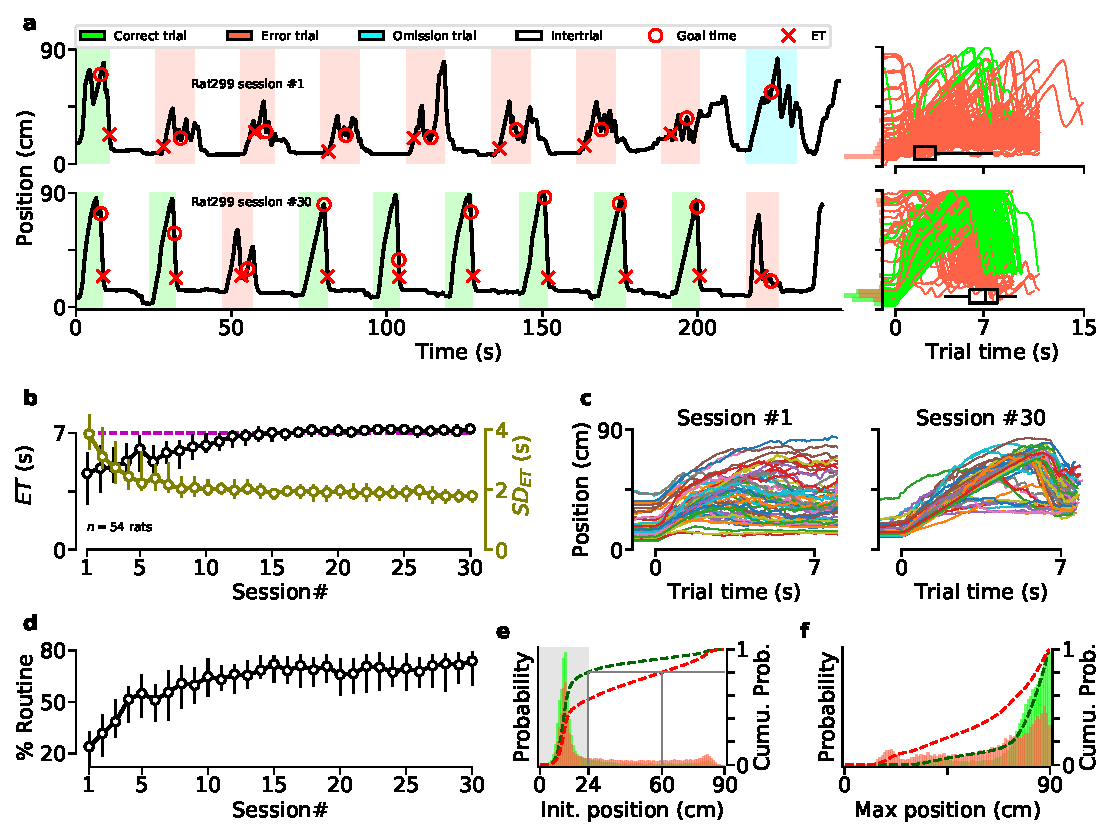
\includegraphics[width=.8\linewidth]{ch-time/figures/CtrlTrd.pdf}
      \caption[Control Condition]
      {\textbf{Most animals developed a unique stereotyped motor sequence.}
      \textbf{a)}
      \textit{Left}: illustration of an animal's trajectory on the treadmill during 9 consecutive trials of the 1st (\textit{top}) and 30th (\textit{bottom}) training sessions.
      On the y-axis, 0 and 90 indicate the treadmill's front (reward port) and rear wall, respectively.
      \textit{Right}: trajectories for all trials during the 1st (\textit{top}) and 30th (\textit{bottom}) sessions (same animal as in left panels).
      Distributions of initial positions for correct (green) and error (red) trials are shown on the y-axis.
      Black horizontal boxplots depict entrance time range (center line, median; box, 25th and 75th percentiles; whiskers, 5th and 95th percentiles).
      \textbf{b)}
      Median entrance time ($ET$) in the reward area for the first 30 daily training sessions.
      Circles indicate group median and error bars, the median range (25th and 75th percentiles) across animals for $ET$ and on the right y-axis,$SD$ of $ET$~($SD_{ET}$) values.
      The dashed magenta line shows the goal time (7~s).
      \textbf{c)}
      Median trajectory of all the trials for the 1st (\textit{left}) and 30th (\textit{right}) training sessions.
      Each line represents a single animal~($n=54$).
      \textbf{d)}
      Session-by-session percentage of trials during which animals performed the stereotyped front-back-front routine (see \nameref{ch:methods:methods}).
      Circles indicate group median and error bars, the median range across animals (25th and 75th percentiles).
      \textbf{e)}
      Probability distribution function~(PDF) of the position of the animals at the beginning of each correct (green) and error (red) trial, from sessions \#20 to \#30.
      Dashed lines represent cumulative distribution functions (right y-axis).
      The gray area indicates that in trained animals,~80\% of correct trials began with the animal located near the front of the treadmill.
      \textbf{f)}
      PDF of the maximum position along the treadmill reached by animals before crossing the beam~($=ET$).
      Only trials in which animals were initially located in the front of the treadmill (gray area in panel~e) were included.
    }
    \label{fig:time:CtrlTrd}
    \end{center}
  \end{figure}
The percentage of trials for which animals used this motor routine increased during learning (\Autoref{fig:time:CtrlTrd}{d}).
Even though a strong preference for the reward area was observed for both correct and error trials, the probability to start a trial in the front portion of the treadmill was higher for correct trials compared to error trials (\Autoref{fig:time:CtrlTrd}{e}), a tendency that developed progressively during training (\autoref{fig:appendix:initPos}).
\par
In addition, if an animal started a trial in the front portion of the treadmill, the probability of reaching the back of the treadmill was higher in correct trials than in error trials (\Autoref{fig:time:CtrlTrd}{f}), further confirming that correct trials were mostly those in which the animals followed the wait-and-run routine and effectively reached the back of the treadmill before running forward toward the reward area.
However, a significant fraction of the animals (14 out of 54) did not develop such a strategy (\Autoref{fig:time:CtrlTrd}{c right}, \Autoref{fig:appendix:BadCtrl}{a}).
Compared to these animals, those regularly following the wait-and-run routine entered the reward area later, demonstrated reduced variability, and an increased percentage of correct trials (\Autoref{fig:appendix:BadCtrl}{b-d}).
Note that one cannot exclude the possibility that animals categorized as \textit{other} in \autoref{fig:appendix:BadCtrl} also used a more subtle stereotyped motor routine not captured by tracking the average body position along the treadmill length.
Anyway, the above results suggest that following a front-back-front trajectory through the ``wait-and-run'' routine is the most reliable strategy to accurately respect the 7~s-rule of the task.


\subsection{Variable Speed Condition}
\label{ch:time:varSpeed}

It could be argued that task parameters (length of the treadmill, its speed, position of the infrared beam,\dots) favored the development of this stereotyped strategy.
Indeed, depending on the initial position of the animal body at trial onset, it can take up to~7 or~8 seconds for the animals to passively reach the back of the treadmill (\Autoref{fig:time:CtrlTrd}{a}) after which they can start running toward the reward area without the need to estimate time at all!
Thus, in the following experiments, we examined how accurately animals respected the GT, when distinct task parameters were modified in a way that hampered the use of this simple wait-and-run motor routine.
First, we trained a new group of rats in a version of the task in which, for each trial, the speed of the treadmill was randomly selected from a uniform distribution between~5 and 30~cm/s (\Autoref{fig:time:varTrd}{a}).
\begin{figure}[bt!]
  \begin{center}
    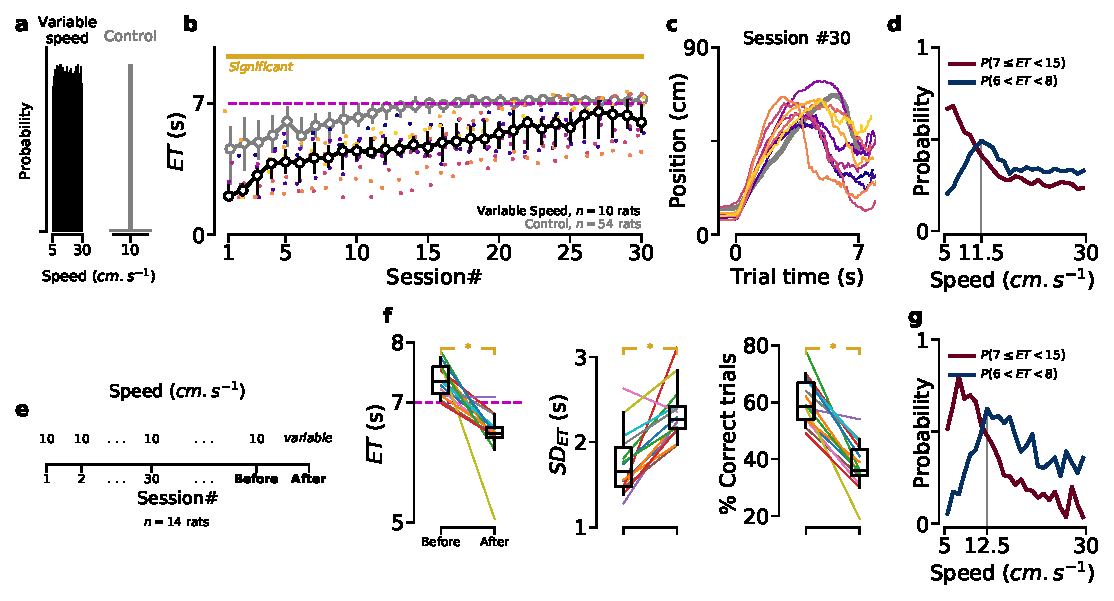
\includegraphics[width=\textwidth]{ch-time/figures/VarTrd.pdf}
    \caption[Variable Speed Condition]
    {\textbf{Decreased temporal accuracy when the treadmill speed randomly changed every trial.}
    \textbf{a)}
    For each trial, treadmill speed was either fixed at 10~cm/s (control condition, same data as in \autoref{fig:time:CtrlTrd}), or randomly selected from a uniform distribution between 5 and 30~cm/s (variable speed condition).
    \textbf{b)}
    Median \gls{et} for animals trained in the variable speed (black), and control (gray) conditions.
    Colored dots indicate individual ``variable speed'' animals.
    Golden line in this manuscript shows statistically significant differences between groups (permutation test).
    \textbf{c)}
    Median trajectory of variable speed animals in session \#30 (same colors as in panel~b).
    \textbf{d)}
    Probability of correct (7~$\leq$~ET~$<$~15~s) and precise (6~$<$~ET~$<$~8~s) trials, given the treadmill speed, for variable speed animals (session~\# $\geq$20).
    \textbf{e)}
    After extensive training in the control condition, some animals ($n=14$) were tested in a probe session with variable speed.
    \textbf{f)}
    Median \gls{et} (\textit{left}), $SD$ of ET (\textit{middle}), and percentage of correct trials (\textit{right}) in the sessions before and after the change in the speed condition.
    Each line represents a single animal.
    Asterisks indicate significant differences (non-parametric paired comparison).
    \textbf{g)}
    Similar to panel~d, for the data collected from the probe session.
  }
  \label{fig:time:varTrd}
  \end{center}
\end{figure}
We found that, during the course of training, these animals consistently failed to wait as long as the animals trained in the control version of the task (``control'' group, \Autoref{fig:time:varTrd}{b}).
Still, the average trajectories of animals extensively trained in this ``variable speed'' condition revealed that they followed a front-back-front trajectory (\Autoref{fig:time:varTrd}{c}).
Accordingly, the probability of performing a correct trial, given different speeds, fell rapidly from~5 to~$\sim$15~cm/s and was lowest for the fastest treadmill speeds (\Autoref{fig:time:varTrd}{d}).
Indeed, it shows that when the treadmill speed was fast, performing the wait-and-run strategy resulted in error trials, as animals reached the back region of the treadmill earlier, compared to when the treadmill speed was slow.
Interestingly, we also found that the probability of precise approaches, i.e., entering the reward area at the~GT$\pm 1$~s sharply peaked for a treadmill speed (11.5~cm/s) that is suitable to perform the wait-and-run motor sequence (\Autoref{fig:time:varTrd}{d}, notice that this speed is very close to the speed in the control condition).
Finally, when rats extensively trained in the control version of the task underwent a single probe session with variable speed (\Autoref{fig:time:varTrd}{e}), all measures of performance dropped significantly (\Autoref{fig:time:varTrd}{f}).
Examining the probability of correct trials and precise approaches given the treadmill speed, resembled those of animals well-trained in the variable condition and suggested that rats kept performing the wait-and-run routine they previously learned in the control condition (compare \Autoref{fig:time:varTrd}{g} and \Autoref{fig:time:varTrd}{d}).


\subsection{No-Timeout Condition}
\label{ch:time:nto}

In the control condition, $\sim$80\% of correct trials started while animals were in the reward area (\autoref{fig:time:CtrlTrd}e).
If rats relied on an internal clock-based algorithm to accurately time their entrance in the reward area, they should adapt relatively easily to a perturbation of their initial starting position.
To test this prediction, we trained a group of rats in a modified version of the task that penalized them when they started the trials in the front region of the treadmill.
This was done by activating the infrared beam as soon as the motor was turned on (in the control condition, the infrared beam was inactive during a \textit{timeout} period that lasted 1.5~s after treadmill onset).
In this "no-timeout" condition, error trials corresponded to $ET$s occurring between 0 and 7~s after motor onset (\autoref{fig:time:ntoTrd}a).
 \begin{figure}[bt!]
  \begin{center}
    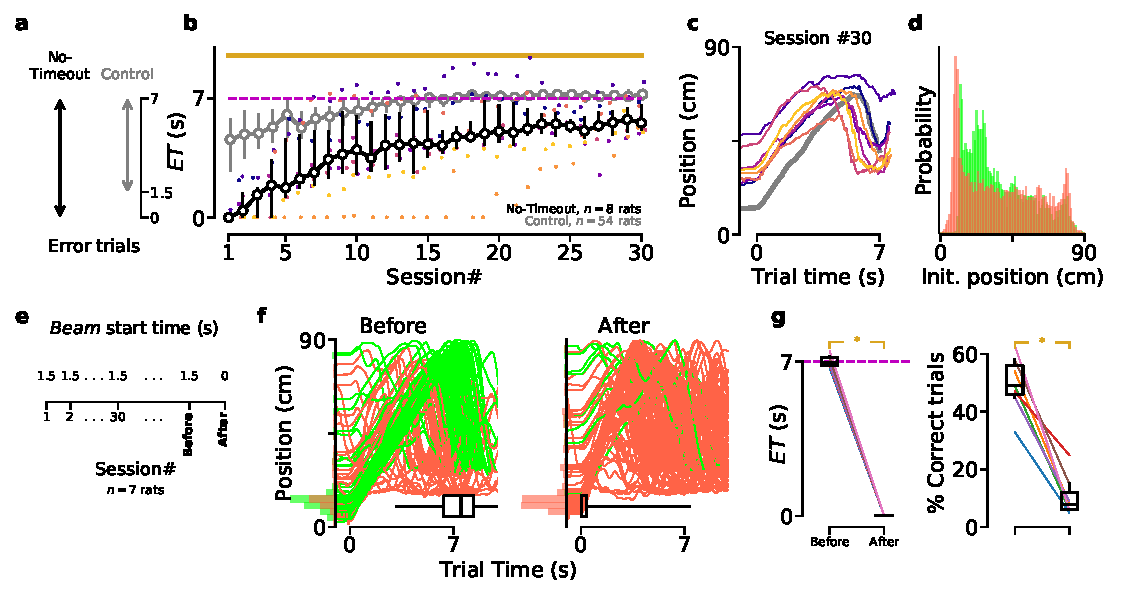
\includegraphics[width=.8\linewidth]{ch-time/figures/NToTrd.pdf}
    \caption[No-Timeout Condition]
    {\textbf{Decreased temporal accuracy when animals are penalized for starting trials in the reward area.}
    \textbf{a)}
    In the control condition, animals had a 1.5~s timeout period to leave the reward area after motor onset.
    In ``no-timeout'' condition, crossing the infrared beam any time before 7~s registers as an error trial.
    \textbf{b)}
    Median $ET$ for animals trained in the no-timeout (black), and control (gray) conditions.
    Colored dots indicate performance for individual no-timeout animals.
    \textbf{c)}
    Median trajectory of no-timeout animals (same colors as in panel~b) in session~\#30.
    \textbf{d)}
    PDF of the no-timeout animals' positions at the beginning of each trial, from sessions~\#20 to~\#30.
    \textbf{e)}
    After extensive training in control condition, animals ($n=7$) were tested in a no-timeout probe session, in which the beam started at the beginning of the trial, rather than 1.5~s later.
    \textbf{f)}
    Trajectories of a representative animal in the last control session (\textit{left}), and the probe session (\textit{right}).
    \textbf{g)}
    Median $ET$s (\textit{left}), and percentage of correct trials (\textit{right}) in the sessions immediately before and after the change in beam start time.
    Each line represents a single animal.
    Asterisks indicate significant differences (non-parametric paired comparison, see \autoref{ch:methods:tech}).
    }
    \label{fig:time:ntoTrd}
  \end{center}
\end{figure}

Animals trained in this condition never reached the level of timing accuracy displayed by animals in the control condition (\autoref{fig:time:ntoTrd}b).
Still, no-timeout animals followed a front-back-front trajectory (\autoref{fig:time:ntoTrd}c) and correct trials were associated with the animals starting the trials just behind the infrared beam (\autoref{fig:time:ntoTrd}d).
The stereotyped reliance on the wait-and-run strategy was also demonstrated by the fact that rats extensively trained in control condition kept performing the exact same trajectory when tested in a single probe session under no-timeout condition, leading to a sharp decrease in performance (\autoref{fig:time:ntoTrd}e-g).
\par
\begin{figure}[!bt]
  \begin{center}
    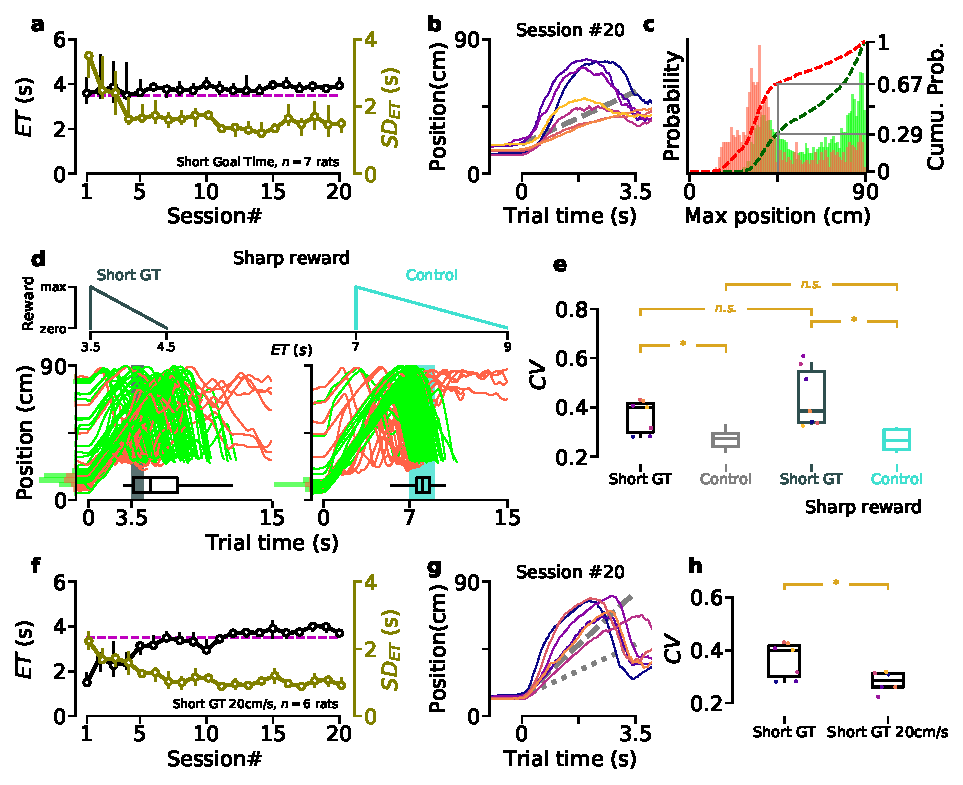
\includegraphics[width=\textwidth]{ch-time/figures/ShortGT-SharpTrd.pdf}
    \caption[Short~GT \& Sharp Conditions]
    {\textbf{Decreased temporal accuracy when the goal time is short.}
    \textbf{a)}
    Median $ET$ during training ($GT=3.5$~s).
    \textbf{b)}
    Median trajectory of ``short~GT'' animals after training.
    Colored lines indicate performance of individual animals.
    Dashed line's slope shows the treadmill speed (10~cm/s).
    \textbf{c)}
    PDF of the maximum position of the short~GT animals for correct (green) and error (red) trials.
    Dashed lines represent cumulative distributions (right y-axis).
    Data collected from session~\#~$\geq15$.
    \textbf{d)} 
    Sharp reward condition applied to short~GT and control experiments.
    \textit{Top}: reward profiles of the sharp reward condition applied to the short~GT (dark) and the control experiments (light).
    \textit{Bottom}: trajectories of 2 illustrative sessions after extensive training in sharp condition (\textit{left}, short~GT; \textit{right}, control).
    Highlighted areas indicate the reward window.
    \textbf{e)}
    Coefficient of variation~($CV$) for short~GT and control experiments with normal (the first two boxes), and sharp (the last two boxes) reward profiles.
    Data collected and averaged once performance plateaued.
    Short~GT vs. Control: $p<0.0001$;
    Sharp short~GT vs. Sharp control: $p<0.0001$.
    \textbf{f)}
    Similar to panel~a, for another group of animals trained to wait 3.5~s while the treadmill speed was 20~cm/s.
    \textbf{g)}
    Similar to panel~b, for animals of panel~f.
    Dashed line's slope shows the treadmill speed (20~cm/s).
    Dotted line's slope shows 10~cm/s.
    \textbf{h)}
    $CV$ for short~GT and short~GT at 20~cm/s conditions (same colors as in panels~b,~g).
    Data collected and averaged once performance plateaued.
    }
    \label{fig:time:shortSharp}
  \end{center}
\end{figure}
We next examined how animals behaved when the goal time (GT) was set to 3.5~s (\autoref{fig:time:shortSharp}), a condition in which the performance of the wait-and-run strategy would lead to late $ET$s (and smaller rewards) because it can take up to $\sim$8~s for the animals to passively travel from the front to the rear portion of the treadmill.
Animals successfully entered the reward area after 3.5~s and reduced their variability across training sessions (\autoref{fig:time:shortSharp}a) but as a group, they displayed an increased $ET$ variability compared to animals trained in the control condition, with GT set 7~s (\autoref{fig:time:shortSharp}e).
From the averaged trajectories of "short GT" animals measured once their performance plateaued, it appeared that 3 subjects out 7 followed a front-back-front trajectory by running toward the rear portion of the treadmill.
The other 4 animals remained still when the treadmill was turned on and tried to run forward before reaching the rear wall (\autoref{fig:time:shortSharp}b).
Interestingly, after training, in 67\% of the error trials, the rats started running forward before reaching the middle of the treadmill (\autoref{fig:time:shortSharp}c, compare with red histogram in \autoref{fig:time:CtrlTrd}f).
Conversely, after initiating a trial in the reward area, the probability of visiting a deeper portion of the treadmill was much stronger in correct than error trials, reinforcing the idea that accurate timing was accomplished by exploiting the most salient physical features of the environment (\autoref{fig:time:shortSharp}c).
Accordingly, the 3 rats that followed the front-back-front trajectory were less variable than those that passively stayed still before running toward the reward area from the middle of the treadmill (\autoref{fig:time:shortSharp}e, same color code as in panel~b).
In addition, among animals trained in the short goal time condition, we found that the magnitude of the backward displacement on the treadmill was negatively correlated with $ET$ variability ($r=-0.49, p=2.7\times 10^{-3}$, Pearson's correlation).
In the short GT condition, animals became proficient more rapidly than in the control condition (compare \autoref{fig:time:shortSharp}a with \autoref{fig:time:CtrlTrd}c).
Could the increased $ET$ variance when the GT is 3.5~s be explained by the fact that the task is easier in this condition and that animals do not need to be very precise?
To test this possibility, we increased the penalty for early $ET$s and decreased reward size for late $ET$s.
In this "sharp reward" condition, the performance of the animals trained in the short GT was even more variable (\autoref{fig:time:shortSharp}d-e).
This result confirms that under short GT condition animals can not accurately time their entrance in the reward area.
Finally, another group of animals was trained with GT set to 3.5~s and treadmill speed at 20~cm/s (i.e., twice as fast, such as following the front-back-front trajectory through the wait-and-run motor sequence would lead to $ET$s close to the GT, \autoref{fig:time:shortSharp}f).
These animals displayed reduced $ET$ variability compared to animals trained at 10~cm/s, and after treadmill onset they stayed immobile until reaching the end of the treadmill, similar to animals trained in the control condition (\autoref{fig:time:shortSharp}g,h).
\par
\begin{figure}[bt!]
  \begin{center}
    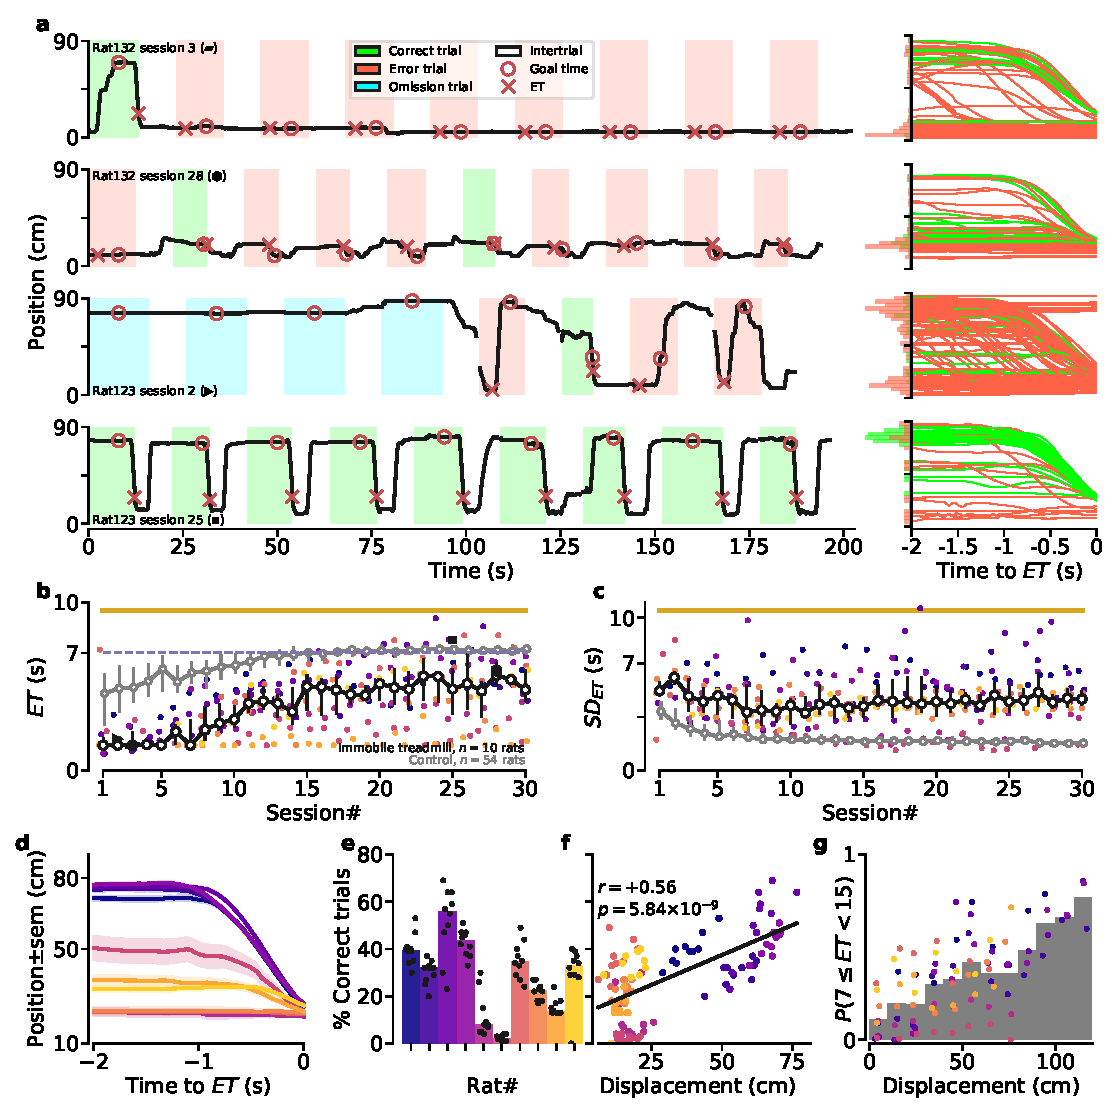
\includegraphics[width=.8\linewidth]{ch-time/figures/ImmTrd.pdf}
    \caption[Immobile treadmill]
    {\textbf{Performance of animals trained while the treadmill remained immobile.}
    \textbf{a)}
    \textit{Left}: illustrations of the positions of two animals on the immobile treadmill for~9 consecutive trials, early (\textit{1st row:}~Rat~\#132-session~\#3, \textit{3rd row:} Rat~\#123-session~\#2) and late (\textit{2nd row:} Rat~\#132-session~\#28, \textit{4th row:} Rat~\#123-session~\#25) during training.
    \textit{Right}: trajectories for all the trials of the corresponding sessions on the left, aligned to the $ET$.
    Distributions of positions 2~s before $ET$, for correct (green) and error (red) trials are shown on the y-axis.
    \textbf{b)}
    Median $ET$ across sessions for "immobile treadmill" animals.
    Filled black markers correspond to the sessions illustrated in panel~a.
    \textbf{c)}
    Similar to panel~b, for the standard deviation of entrance times ($SD_{ET}$).
    \textbf{d)}
    Median trajectory aligned to $ET$ of each "immobile treadmill" animal (only correct trials from sessions~\#20 to~\#30 are considered; shaded regions denote standard error).
    \textbf{e)}
    Median percentage of correct trials for each immobile treadmill animal (same sessions as in panel~d).
    Each dot represents one session.
    \textbf{f)}
    Repeated measures correlation between the percentage of correct trials and average displacement during a session.
    Each dot represents one session.
    \textbf{g)}
    PDF of a correct trial, given the displacement of an animal.
    Each dot represents the average probability for an individual animal, during a single session.
    \textbf{(e-g)}
    Analyses based on the same sessions as in panel~d.
    Individual animal color code is preserved in panels~b-g.
    }
    \label{fig:time:ImmTrd}
  \end{center}
\end{figure}

The above results suggest that, in a task requiring animal to produce a motor response according to a fixed temporal constraint, the possibility to perform a stereotypical motor sequence adapted to salient features of the environment (here, taking advantage of the full treadmill length and its physical boundaries) critically determines temporal accuracy.
To further investigate this idea, we trained a group of animals in a version of the task in which the treadmill was never turned on (trial onset was signalled by turning the ambient light on).
In this condition, animals displayed a strong impairment in respecting the GT, compared to animals trained in the control condition (\autoref{fig:time:ImmTrd}a,b).
On average, animals reached the reward area later and later across sessions but displayed a constant high variability in $ET$ (\autoref{fig:time:ImmTrd}c).
We also noticed that correct trials preferentially occurred when animals crossed the treadmill from the rear wall to the reward area (Video 3, \autoref{fig:time:ImmTrd}a,d,e).
Accordingly, after extensive training, a robust correlation was observed on a session by session basis between the percentage of correct trials and displacement of the animal on the treadmill (\autoref{fig:time:ImmTrd}f).
Moreover, the probability of a correct trial increased for higher values of displacement (\autoref{fig:time:ImmTrd}g).
\par
\begin{figure}[bt!]
  \begin{center}
    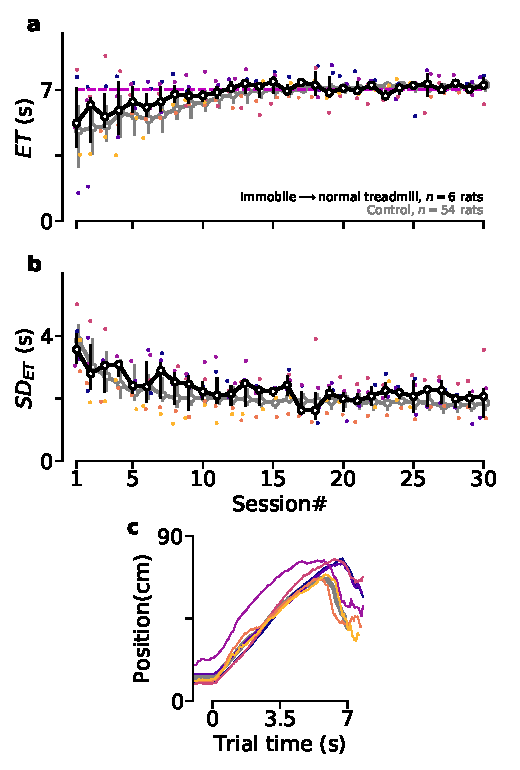
\includegraphics[width=.4\linewidth]{ch-time/figures/Imm2CtrlTrd.pdf}
    \caption[Immobile animals relearning the task]
    {\textbf{Lack of temporal knowledge transfer across task protocols.}
    After extensive training on the immobile treadmill, animals were trained under normal conditions (GT$=7$~s, treadmill speed$=10$~cm/s).
    \textbf{a)}
    Median $ET$ across sessions in control condition.
    \textbf{b)}
    Similar to panel~a, for the standard deviation of entrance times ($SD_{ET}$).
    \textbf{c)}
    Median trajectory of the individual animals after relearning the task in the control condition.
    \textbf{a-c)}
    Individual animal color code is preserved in all panels.
    }
    \label{fig:time:Imm2Ctrl}
  \end{center}
\end{figure}

Lastly, animals trained in the immobile treadmill condition during several weeks were challenged in the control condition (i.e., by simply setting the treadmill speed at 10~cm/s).
These animals improved their behavior at the same pace and with the same wait-and-run routine as na\"ive animals (\autoref{fig:time:Imm2Ctrl}a-c).
Thus, animals that previously learned to wait in one version of the task did not learn faster than na\"ive animals when challenged in a second version of the task with distinct movement requirement but identical GT, demonstrating again that task proficiency relied primarily on the acquisition of a motor sequence rather than an internal knowledge of time.